\section{Redes de eSalud}

Conjunto de nodos relacionados con capacidad operativa de brindar servicios de eSalud, garantizando atributos de calidad, estandarización, interoperabilidad, privacidad y seguridad \cite{wilson2017}. La arquitectura base de cada nodo de la red es de tipo agregado con \textit{micronodos} agrupados funcionalmente para brindar un servicios son consumidos por otros nodos,creando estructuras funcionalmente complejas.En este sistema los nodos de más alto nivel de abstracción son lo que tienen capacidad de ofrecer servicios de eSalud.

\begin{figure}
 \centering
 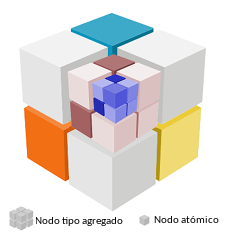
\includegraphics[width=80mm, height=83mm]{concepto_red_esalud.png}
 \caption{Vista conceptual de la arquitectura de una red de eSalud en OpenSITEM}
 \label{elementosred}
\end{figure}

De acuerdo a las recomendaciones del grupo GITEM, la descripción de la arquitectura de cada nodo - así como la de la red, puede obtenerse de manera emergente utilizando métodos tales como el Architecture Development Method (ADM) de The Open Group o similares. Se recalca que OpenSITEM no es una plataforma para prestación de servicios de eSalud sino para la descripción de nodos de la red - a diferentes niveles de abstracción, a partir del modelo de agregación. 

\subsection{Caracterización de Nodos para Redes de eSalud}

Las redes de eSalud incluyen nodos de diferentes tipos, por ejemplo, médicos, tecnológicos, de recurso humano, financiero, estratégico, de organización, de política y de infraestructura \cite{ops2011},\cite{oms2016}, \cite{ituoms2012}. En el estudio de campo el equipo de diseño y planeación de redes de eSalud, se encontró con el obstáculo de no disponer de información de calidad de los nodos potenciales que harían parte de la red. Por esta razón y con el objetivo de crear una matriz de comparación, se propuso un \textit{reducido} de nodos\footnote{El reducido es un conjunto finito de nodos con capacidad de entregar una funcionalidad contractualmente definida relacionada con la eSalud} y una descripción de la arquitectura de cada uno de ellos, de tal manera que se pudiese recopilar datos basados en modelos de información.

Al definir el resultado se planteó que un servicio - con posibilidad de ser implementado en un modelo de eSalud, requiere de la integración de nodos. En OpenSITEM existen dos tipos de nodos: (1) atómicos: aquellos que ofrecen un servicio cohesivo que no abarca un caso de uso de dominio  y (2) agregados: que articulan nodos (atómicos o agregados) para brindar capacidad funcional a nivel de caso de uso de negocio. Si se considera que el modelo de dominio gira en torno a los servicios de eSalud, el nodo agregado que lo provee se denominará \textit{macronodo}.

Un nodo atómico está caracterizado por atributos (propiedades) e interfaces. Estás últimas son los puntos de acceso en donde los servicios del nodo son expuestos para ser consumidos \cite{theopengroup2016}. Un nodo agregado está definido por el conjunto de atributos de los nodos que lo componen y las interfaces que surgen de la interoperabilidad de dichos nodos. Un nodo puede pertenecer a uno o más agregados razón por la cual un nodo - atómico o agregado, goza de alta cohesión y bajo acoplamiento como patrón principal\footnote{En el mayor grado en que se cumplan estos patrones más simple resulta la caracterización de la red.}.

Otro aspecto que se utiliza para la descripción de los nodos es la categoría o clase a la cual pertenece. Debido a que la arquitectura de la red puede ser abordada desde distintos puntos de vista, un nodo puede tener asociada uno o varias categorías. Por ejemplo, el modelo de componentes que propone la OMS\ref{Subcomponentes} podría definir las categorías de clasificación de los nodos, posterior a ello si surge otro modelo o se edita el actual, los nodos podrían adaptarse para mantener las relaciones y crear unas nuevas. El grupo de investigación desarrolla OpenSITEM enfocado en la caracterización multicategoría de los nodos en redes de salud, tomando como modelo de mayor nivel de abstracción en propuesto por la OMS y uno de baja abstracción con categorías: médica, tecnológicas, administrativa, humana y financiera. Sin embargo, debido al perfil de profesionales que han participado en el desarrollo, los nodos de la categoría tecnológica han sido mejor caracterizados hasta el momento.

\begin{figure}
 \centering
 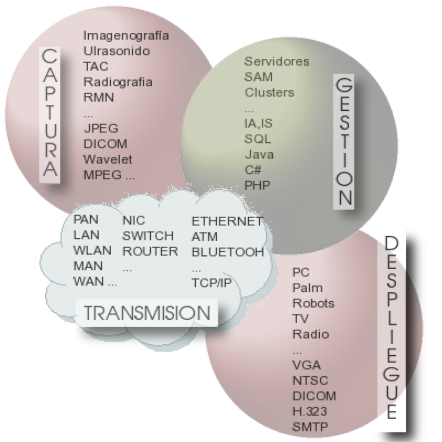
\includegraphics{red_1.png}
 \caption{Componentes en un Sistema de eSalud. Fuente: OMS/ITU}
 \label{subcomponentes}
\end{figure}

\subsection{Subsistemas en Una Red de eSalud}

El grupo GITEM considera que una red de eSalud está compuesta por cuatro subsistemas:

\begin{itemize}
 \item \textbf{Subsistema de Captura de datos:} Conformado por los dispositivos de hardware, los protocolos y aplicaciones software que trabajan conjuntamente para transformar información médica en datos susceptibles de ser administrados usando técnicas digitales.
 \item \textbf{Subsistema de Transmisión de Datos:} Hacen parte de este subsistema los dispositivos de hardware, las tecnologías de interconexión, los protocolos y aplicaciones que permiten estructurar redes de transmisión de datos digitales de una manera fiable en tiempos aceptables para un servicio específico.
 \item \textbf{Subsistema de Gestión de Información:} Dispositivos de hardware - computadores, sistemas de almacenamiento masivo, etc; y  sistemas de información que almacenan, procesan, distribuyen, analizan, integran y producen información con base en los datos de los subsistemas de captura, históricos y de pronóstico.
 \item \textbf{Subsistema de Despliegue de información:} Elementos de hardware (pantallas, transductores, sistemas de audio, etc), aplicaciones software y protocolos asociados que permiten recibir y reproducir información médica. 
\end{itemize}

Todos ellos  sirven como plataforma para determinar cierta organización para la definición de tipos de nodos. 